\section{Overview}

%% Update tenses

The World Wide Lightning Location Network (WWLLN) is used to measure the normalized lightning electric field at three network stations in order to examine the sferic attenuation between the stroke and the station.
The electric field measurements are normalized to the radiated very low frequency (VLF) stroke energy to allow direct comparisons of the many stroke-station paths seen by WWLLN.
WWLLN observes a strong dependence of VLF propagation on magnetic azimuth similar to past work.
From WWLLN the average attenuation over the water of eastward-propagating sferics is found to be $1.13\pm0.35$~dB/Mm during the day and $0.71\pm0.68$~dB/Mm at night, with westward-propagating sferics having average attenuation rates of $2.98\pm0.68$~dB/Mm and $2.66\pm0.39$~dB/Mm for day and night respectively.

%% Transition

%% MM: Add a quick summary of the Wait and Spies theory for why there is the magnetic asymmetry.

Past experimental work has shown a strong dependence of VLF attenuation on the magnetic azimuthal angle of propagation.
\citet{Wait1960a} present a theoretical background for why the attenuation changes with azimuth.
By measuring the signal strength from the same nearly antipodal transmitter along the short and long great circle path, \citet{Crombie1958} found less attenuation for the eastward propagating signals.
Similarly \citet{Taylor1960a} showed that eastward propagating VLF waves have 1 -- 3 dB/Mm less attenuation than westward propagating waves.
Recently \citet{Jacobson2012} used negative cloud-to-ground strokes to examine ionospheric reflectance and also found a strong azimuthal dependence to the measurements.

The past work has examined stationary VLF transmitters with either a few receivers or one moving receiver.
Recent work by \citet{Burkholder2013} utilized the World Wide Lightning Location Network (WWLLN) to examine how eastward and westward propagating VLF sferics couple into the ionosphere.
This work motivated us to use the many stroke-receiver paths of WWLLN to study the azimuthal dependence of VLF propagation within the Earth-ionosphere waveguide.

The global coverage of the network allows for many long range stroke-receiver paths with which to estimate VLF attenuation rates.
The sferic attenuation for a single station can be found with WWLLN by comparing the stroke energies measured by the network to the RMS electric field measured at a single WWLLN station.
Using WWLLN allows for the azimuthal propagation effects to be examined at all magnetic azimuths for both all-night and all-day paths.
The measured electric fields and observed attenuation rates can be directly compared to the theoretical predictions of \citet{Wait1960a} and \citet{Taylor1960a}.
%% Page 209-210
By examining the propagation it is shown that WWLLN captures the effects of propagation and that the theories are applicable for non-stationary transient sources.

\section{Path Selection}

To examine eastward and westward propagation three WWLLN stations were chosen based on their island locations: Suva, Tahiti, and Honolulu.
These stations were selected as a majority of their stroke-receiver paths are over water, so the effects of variable ground conductivity can be ignored. 

The WWLLN energy calculation uses the LWPC code, that accounts for eastward and westward propagation.
However each WWLLN energy measurement is the median energy of several WWLLN stations, so by selecting strokes with a similar number of stations to the east and west the azimuthal dependence computed by LWPC can be minimized.
There is allowed to be at most 25\% more WWLLN stations to the east or west of a located stroke, where this abundance is defined by: $|n_{east} - n_{west}| / n$.
For example, a located stroke with 1 station to the north, 2 east, and 3 west will have a westward abundance of 16.7\% and would be included in the analysis.

With these three stations the WWLLN data are reduced to only consider sferics that crossed at most 5\% land, and propagated in either 95\% day or night ionospheric conditions.
The stroke energy uncertainty (median absolute deviation of contributing stations, see \citet{Hutchins2012}) is limited to a maximum of 10\%.
Further the data are reduced by selecting only strokes with a similar number of locating WWLLN stations situated to the east and west as described above.
These requirements reduce the stroke-receiver paths in the WWLLN dataset to 0.2\% of the total paths for each station, where 87\% occur during the day and 13\% occur at night.
This resulted in over $2\times10^6$ total stroke-receiver paths used in this study.

The subset of data contains the RMS electric field at each station, the distance to the strokes, and the VLF energy of the stroke.
VLF stroke energies and station measured electric fields both vary over several orders of magnitude.
All station electric fields (in units of $1 \mu V m^{-1}$) are normalized by the square root of the stroke energy (in $J$) to allow for direct comparisons between differing source energies.
The stroke energy normalization gives the electric field in dB above $1 \mu Vm^{-1}/J^{1/2}$.
Changes in the normalized electric field with stroke distance gives the attenuation of the lightning sferic for that distance interval, reported as the dB/Mm decrease. 

Normalized field values are grouped into 45$^\circ$ azimuth and 500~km distance bins.
An example of all of the distance bins for a given azimuth for one station is shown in Figure~\ref{azimuth:fig:azimuthCalculation} (northwestward-propagation during the day for Honolulu station).
Each distance bin has a distribution of normalized field values with the spread a result of differing ionospheric conditions, uncertainty in the energy measurements, and changes in ground conditions at the station.
Because of this spread the median value of the normalized field is used for each distance-angle combination (shown as the solid black line).
At least 15 strokes are required for each distance bin at a given azimuth in order to calculate a reasonable median.
The magnetic azimuth used is the average magnetic azimuth over the path of wave propagation.

 \begin{figure}[h!t]
   \centering
   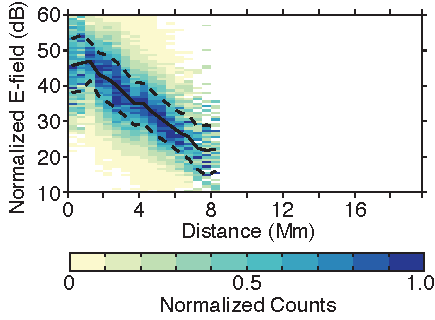
\includegraphics[scale=1]{Azimuth/Figures/azimuthCalculation.pdf} 
   \caption{Normalized electric field values for the 315$^\circ$ azimuth bin for the Honolulu station during the day.
   	Counts are normalized to the maximum value in each distance bin.
	The median (solid) and median absolute deviation (dashed) values are plotted on top of the distribution.
	Distances with less than 15 total strokes are not plotted or used.}
   \label{azimuth:fig:azimuthCalculation}
\end{figure}

\section{Azimuthal Dependence}

For the three stations data were used from May 2009 to May 2013, resulting in $2.1\times10^6$ stroke-station paths to analyze.
The results are split into the 8 azimuth octants for day paths and night paths as shown in Figure~\ref{azimuth:fig:azimuth}.
For the three stations the westward propagating waves (green) show higher attenuation (electric field change per unit distance) than for the eastward propagating waves (red).
The attenuation is also seen in the maximum distance that strokes are detected, with night (eastward) paths detectable at farther distances than day (westward) paths.

 \begin{figure}[h!t]
   \centering
   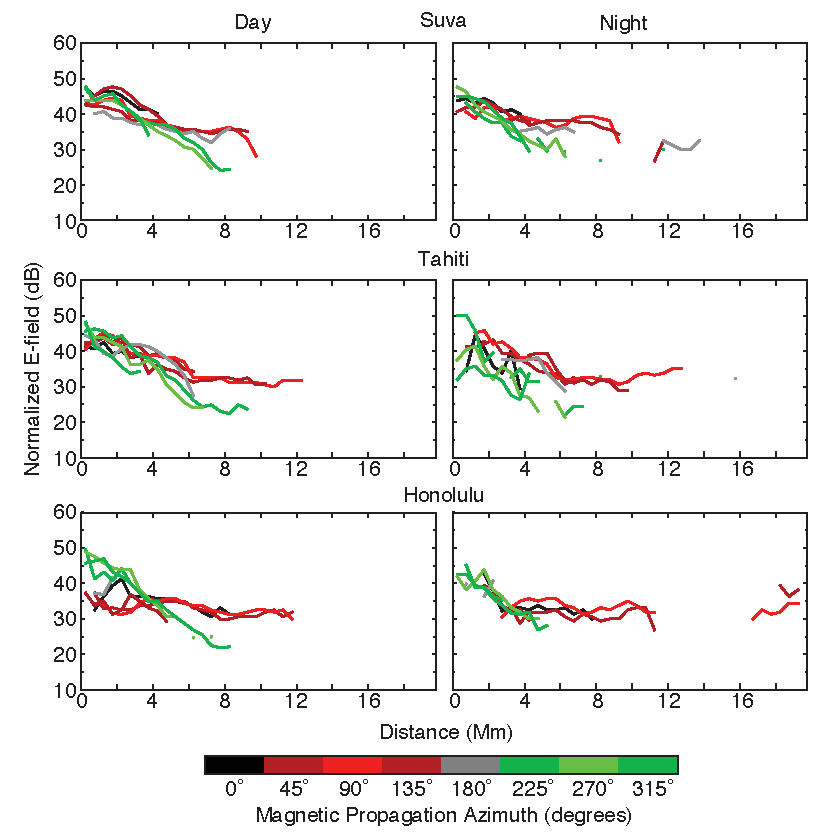
\includegraphics[scale=1]{Azimuth/Figures/e-field_3.pdf} 
   \caption{Station RMS electric field vs distance for Suva, Tahiti, and Honolulu.
   	Electric field is normalized by stroke energy and given in dB above $1 \mu Vm^{-1}/J^{1/2}$.
	Day ionosphere paths are in the left column and night ionosphere paths in the right column.}
   \label{azimuth:fig:azimuth}
\end{figure}

For some stations, such as Honolulu in Figure~\ref{azimuth:fig:azimuth}, the difference between eastward and westward sferics is quite clear during the day at all distance ranges, and between day and night.
For other stations, such as Suva, the difference in propagation direction is not distinct for all azimuths.
Suva and Tahiti stations do not show a differentiation in attenuation until the waves have propagated some distance from the stroke, for example the night strokes for Suva in Figure~\ref{azimuth:fig:azimuth} are indistinguishable until 4~Mm.

In all cases the slopes of the field strength curves in Figure~\ref{azimuth:fig:azimuth} show that the eastward sferics exhibit less attenuation than westward sferics away from the stroke.
In cases like Honolulu the westward sferics initially have a lower normalized electric field, but the attenuation rate of these sferics is still lower than the eastward sferics.
  
The overall behavior of the VLF waves observed by WWLLN can be seen in the compiled station data.
The station-stroke pairs were combined for all stations to give a single dataset of paths, shown in Figure~\ref{azimuth:fig:azimuthAverage}.
The westward sferics in both day and night have similar electric field to the eastward sferics with the distinction developing at greater than 4~Mm from the stroke.
There is a small upturn in field strength as the sferics propagate past 10~Mm because the waves are re-focusing when they cross the halfway point to their antipode.

\begin{figure}[h!t]
    \centering
    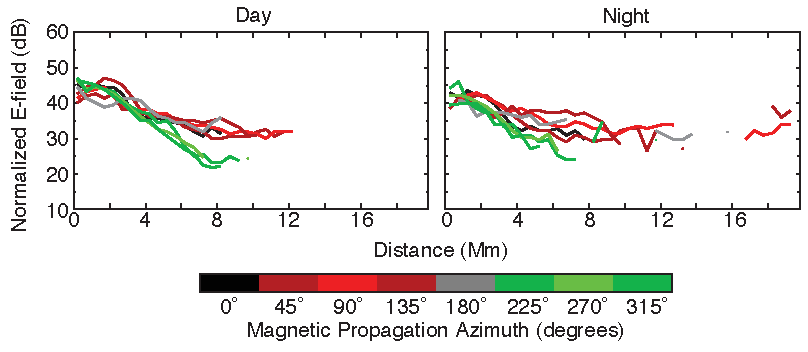
\includegraphics[scale=1]{Azimuth/Figures/azimuthAverage.pdf} 
    \caption{Compiled station normalized electric field for the three selected stations.
    	Shown in dB above $1 \mu Vm^{-1}/J^{1/2}$.}
    \label{azimuth:fig:azimuthAverage}
 \end{figure}

The method for estimating the attenuation and the uncertainty is outlined in Figure~\ref{azimuth:fig:attenuationCalculation} using the station averaged eastward-propagating electric field values as an example (red line in Figure~\ref{azimuth:fig:azimuthAverage}).
The following fitting and smoothing method is used to estimate the attenuation to remove the noise in the direct attenuation (Figure~\ref{azimuth:fig:attenuationCalculation}b). 
First, the normalized electric field versus distance curves are smoothed and fitted to quadratics for the bins that have data, as shown with the dashed line in Figure~\ref{azimuth:fig:attenuationCalculation}a.
Second, the attenuation between each bin of the fit (the slope of Figure~\ref{azimuth:fig:attenuationCalculation}a) is found and shown in Figure~\ref{azimuth:fig:attenuationCalculation}b.
Lastly, the attenuation for a given electric field curve is calculated by the mean of the fitted attenuation where positive attenuation corresponds to a signal loss over distance.
The standard deviation of the attenuation is taken as the uncertainty in the attenuation measurement.
In the example of Figure~\ref{azimuth:fig:attenuationCalculation} the fitted attenuation is $1.13\pm0.35$~dB/Mm whereas the attenuation directly from the data (solid line in Figure~\ref{azimuth:fig:attenuationCalculation}b) is $0.79\pm2.34$~dB/Mm.
The increased uncertainty in the direct attenuation is due to the variations in attenuation between successive 500~km distance bins.
The fitted attenuation is used for all of the following attenuation values.

%% MM: What about geometric effects?  Why not remove them to get a better signal

\begin{figure}[h!t]
    \centering
    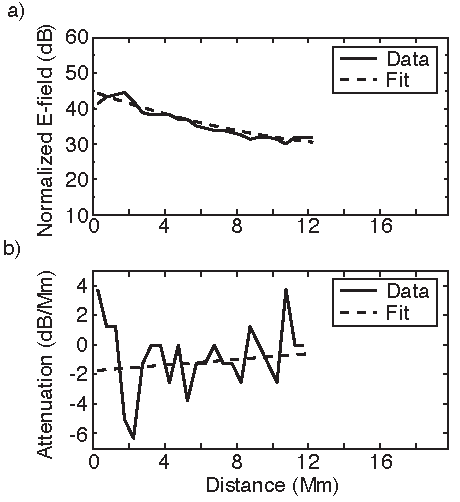
\includegraphics[scale=1]{Azimuth/Figures/attenuationCalculation.pdf} 
    \caption{Method for calculating the attenuation.
    	In a) the normalized electric field vs distance data (solid line) and the fitted quadratic (dashed line).
	In b) the change in electric field with distance step (derivative) for the data (solid line) and the fit (dashed line) normalized to dB/Mm.}
    \label{azimuth:fig:attenuationCalculation}
 \end{figure}

Overall there is an average attenuation of $1.87\pm1.06$~dB/Mm for all azimuths and times.
Within the first 4~Mm of the stroke the attenuation is fairly high for both day and night, with $2.08\pm0.90$~dB/Mm during the day and $2.09\pm1.02$~dB/Mm at night.
Beyond 4~Mm the attenuation decreases to $1.29\pm1.09$~dB/Mm for day and $0.24\pm0.48$~dB/Mm for night.
The 4~Mm cutoff was chosen based on Figure~\ref{azimuth:fig:azimuth} and~\ref{azimuth:fig:azimuthAverage} where the eastward and westward-propagating sferics start to clearly differentiate.
The increased attenuation near the stroke is likely due to the fast decay of higher order modes that cannot propagate far from their source \citep{Wait1970}.

For eastward sferics the average attenuation is $1.13\pm0.35$~dB/Mm and $0.71\pm0.68$~dB/Mm for day and night; for westward sferics attenuation is higher with rates of $2.98\pm0.68$~dB/Mm and $2.66\pm0.39$~dB/Mm for day and night paths.
The difference in attenuation between eastward and westward-propagating sferics is an increase of  1.9~dB/Mm for day and 2.0~dB/Mm for night.
  
\section{Comparisons to Theory}

The azimuthal variability of the WWLLN normalized electric-field attenuation is directly compared to the azimuthal variance predicted by \citet{Wait1960a} in Figure~\ref{azimuth:fig:attenuationTheory}.
The azimuthal variation, P$(\phi)$, is found by comparing the attenuation with the presence of a magnetic field to the attenuation without.
For the WWLLN data the average attenuation of all azimuths is taken as representative of the attenuation with no magnetic field.
The variability of the attenuation rate (in dB/Mm) with magnetic azimuth from \citet{Wait1960a} is approximated as $P(\phi) = - 0.3 \times \text{sin}(\phi) + 1$.

%% MM: does the wait attenuation rats here account for the geometric effect?

\begin{figure}[h!t]
   \centering
   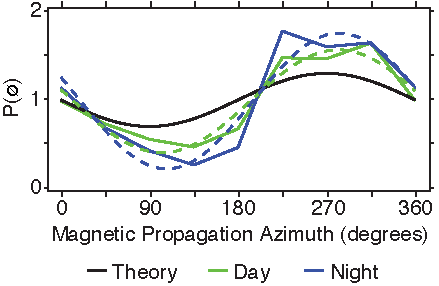
\includegraphics[scale=1]{Azimuth/Figures/attenuationTheory.pdf} 
   \caption{Dependence of attenuation with magnetic azimuth shown as P($\phi$), the attenuation normalized to attenuation with no magnetic field.
   	Shown for \citet{Wait1960a} (black), day paths (green), and night paths (blue).
	The best fit curves are shown as dashed lines.
	Day and night paths are normalized by their mean.}
   \label{azimuth:fig:attenuationTheory}
\end{figure}

The average attenuation azimuthal variation was fit to the same form as the theory ($P(\phi) = - a~\times~\text{sin}(\phi + b) + 1$) with the resulting fits shown in Figure~\ref{azimuth:fig:attenuationTheory}.
The leading coefficient, $a$, gives the relative variation in attenuation with azimuth; how much attenuation rates will change between northward/southward and eastward/westward propagating sferics.
The day attenuation best fit is $P(\phi) = - 0.58 \times \text{sin}(\phi + 348) + 1$ and the night attenuation best fit is $P(\phi) = - 0.76 \times \text{sin}(\phi - 344) + 1$.
Both day and night paths show twice the amplitude relative to the theory ($a_{theory} = 0.3$), with a weaker day dependence and a stronger night dependence, $a=0.58 \pm 0.18$ and $a=0.76 \pm 0.26$ respectively.
On average the day measurements vary from the theory by 19\% and the night measurements by 34\%.

In previous measurements of 3 -- 30~kHz VLF attenuation \citet{Taylor1960a} observed westward VLF paths to exhibit 1-3~dB/Mm more attenuation than eastward paths.
This is in line with the WWLLN measured increase of 1.9-- 2.0~dB/Mm from eastward to westward-propagating sferics.
Similarly the LWPC model shows an attenuation increase of 2~dB/Mm from eastward to westward-propagating sferics for equatorial day paths over the Pacific Ocean.
The model also gives a 28\% to 37\% variability of attenuation between propagation directions, relative to northward propagation, compared to 30\% for \citet{Wait1960a} and 58\% to 77\% for WWLLN.

%% MM: Need to say something definite and original.
%% MM: So are the measurements consistent with theory or not?

\section{Conclusion}

Four years of WWLLN data were used to analyze the normalized VLF electric field from lightning at three island stations, with the variation with magnetic azimuth compared to theoretical results.
The electric fields were used to calculate the average attenuation in the 8 -- 18~kHz band at different propagation azimuths.
The stroke-receiver paths were selected for sferics propagating over at least 95\% water and under either 90\% day or 90\% night ionospheric conditions.

It was found that compared to day propagation, night propagating sferics have higher attenuation close to the stroke ($2.09\pm1.02$) with less attenuation farther out ($0.24\pm0.48$).
Similarly attenuation of night sferics have a higher dependence on magnetic azimuth compared to day sferics.
Variations with magnetic azimuth showed that westward propagation had 1.9 -- 2.0~dB/Mm more attenuation than eastward propagation for both day and night ionospheric conditions.

Combining three optimally placed WWLLN stations allowed for this examination of the azimuthal dependence of VLF attenuation.
Utilizing more of the 70 stations will allow for further investigation of VLF attenuation rates with other path parameters such as ocean salinity, ice, and ground conductivity.
